\section{Marco teórico conceptual}
\label{sec:marco-teorico}

En este capítulo se presentan los conceptos que sustentan el trabajo. Se parte del Procesamiento de Lenguaje Natural, su evolución y sus tareas principales, para ubicar a la traducción automática dentro del campo. Después se describe la Comunicación Aumentativa y Alternativa, el catálogo de pictogramas ARASAAC y la función comunicativa de la traducción de texto a pictogramas. Enseguida se explican las redes neuronales, la arquitectura Transformer y los modelos preentrenados, que son la base técnica del modelo propuesto. Finalmente, se aborda la traducción automática con Transformers y las métricas con las que se evalúa la calidad de una traducción, junto con su adaptación al caso de los pictogramas.

\subsection{Procesamiento de Lenguaje Natural (PLN)}
El Procesamiento de Lenguaje Natural (NLP, por sus siglas en inglés) es la disciplina de la Inteligencia Artificial dedicada a dotar a los sistemas computacionales de la capacidad de comprender, interpretar y generar lenguaje humano de forma automática \cite{bharadiya2023nlp}. 

    De acuerdo a Bharadiya\cite{bharadiya2023nlp}, los orígenes del procesamiento de lenguaje se remontan a enfoques basados en reglas lingüísticas explícitas, diseñadas manualmente por expertos, que buscaban capturar la gramática y la semántica del lenguaje mediante sistemas simbólicos. Con el tiempo, la disciplina evolucionó hacia paradigmas cada vez más dependientes de datos.

\subsubsection{Evolución metodológica del NLP}

La evolución del NLP ha ido cambiando de enfoque como respuesta a las limitaciones y nuevas necesidades. Por ejemplo,los primeros sistemas estaban basados en reglas y por ende dependían de gramáticas formales y diccionarios construidos manualmente por lingüistas computacionales; si bien permitían un control interpretable sobre el comportamiento del sistema, su escalabilidad era limitada, dado que la cobertura de fenómenos lingüísticos crecía linealmente con el esfuerzo humano requerido, y presentaban un mal desempeño frente a la ambigüedad y variabilidad inherentes al lenguaje natural.

Estas limitaciones impulsaron el desarrollo de métodos estadísticos que modelaban el lenguaje como distribuciones de probabilidad obtenidas a partir del análsisi de grandes volúmenes de texto, ejemplos de este paradigma son los modelos de m-gramas y los modelos ocultos de Markov. Sin embargo estos modelos seguían dependiendo en gran medida de ingeniería manual de características, como resultado se buscaron mejoras mediante la incorporación de técnicas de aprendizaje automático clásico y posteriormente de técnicas de aprendizaje profundo. Este último permite que los propios modelos aprendar representaciones a partir del texto de origen sin necesidad de ingeniería manual de características \cite{young2018recent}.

 Las arquitecturas neuronales demostraron una capacidad superior para capturar dependencias contextuales y relaciones semánticas complejas, lo que condujo, en años recientes, a la emergencia de modelos preentrenados sobre volúmenes masivos de texto y posteriormente adaptados a tareas específicas, así como al surgimiento de los denominados Large Language Models (LLM), capaces de exhibir capacidades emergentes de comprensión y generación de lenguaje a una escala sin precedentes en la historia del campo.


\subsubsection{Principales tareas del Procesamiento de Lenguaje Natural}

Hang Li \cite{Li2018} propone una clasificación de cinco tareas principales dentro del procesamiento de lenguaje natural, las cuales son clasificación (classification), emparejamiento (matching), traducción (translation), predicción estructurada (structured prediction) y proceso de decisión secuencial (sequential decision process). La  tabla \ref{tab:five-nlp-tasks} resume dichas tareas.

\begin{table}[H]
\centering
\caption{Cinco tareas del procesamiento de lenguaje natural \cite{Li2018}}
\label{tab:five-nlp-tasks}
\renewcommand{\arraystretch}{1.4}
\setlength{\tabcolsep}{8pt}
\small
\begin{tabular}{@{} >{\raggedright\arraybackslash}p{2.6cm}
                    >{\raggedright\arraybackslash}p{3.2cm}
                    >{\raggedright\arraybackslash}p{2.6cm}
                    >{\raggedright\arraybackslash}p{4.2cm} @{}}
\toprule
\textbf{Tarea} & \textbf{Descripción} & \textbf{Modelo} & \textbf{Aplicaciones} \\
\midrule

Clasificación &
asignar una etiqueta a una cadena &
$s \rightarrow c$ \newline
$s$: cadena, $c$: etiqueta &
clasificación de texto, análisis de sentimientos \\

\midrule

Emparejamiento &
comparar dos cadenas &
$s, t \rightarrow R^{+}$ \newline
$s$: cadena, $t$: cadena \newline
$R^{+}$: valores reales no negativos &
búsqueda, respuesta a preguntas, diálogo de un turno (basado en recuperación) \\

\midrule

Traducción &
transformar una cadena en otra &
$s \rightarrow t$ \newline
$s$: cadena, $t$: cadena &
traducción automática, reconocimiento automático de voz, diálogo de un turno (basado en generación) \\

\midrule

Predicción estructurada &
mapear una cadena a una estructura &
$s \rightarrow [s]$ \newline
$s$: cadena, $[s]$: estructura &
reconocimiento de entidades nombradas, segmentación de palabras, etiquetado gramatical, análisis de dependencias, análisis semántico \\

\midrule

Proceso de decisión secuencial &
tomar acciones en estados dentro de un entorno dinámicamente cambiante &
$\pi: s \rightarrow a$ \newline
$\pi$: política, $s$: estado, $a$: acción &
diálogo de múltiples turnos \\

\bottomrule
\end{tabular}
\end{table}


Entre estas tareas, la traducción automática ocupa un lugar particular por la complejidad que entraña: a diferencia de tareas de clasificación o etiquetado, que operan sobre un espacio de salida acotado, la traducción automática requiere generar una secuencia de salida completa en un espacio diferente. Además de que se debe de preservar simultáneamente el contenido semántico, la estructura sintáctica y las convenciones idiomáticas del idioma destino. 

\subsubsection{Representación computacional del lenguaje}

Para que el lenguaje natural pueda ser procesado por algoritmos, primero debe transformarse en representaciones numéricas. Una de las técnicas más simples es Bag of Words que usa vectores de frecuencia de palabras, ignorando orden y contexto, esta aproximación tiene la desventaja de que sufre alta dimensionalidad, dispersión y nula semántica \cite{murel2023bagofwords}. Otra técnica es TF-IDF, esta pondera por rareza en el corpus, mejorando la discriminación, pero sigue sin captar significado entre términos: por ejemplo, trata palabras como coche y automóvil como entidades completamente independientes, sin reconocer su relación semántica.

Word Embeddings introducen vectores densos y de baja dimensión que sitúan palabras relacionadas cerca, capturando relaciones semánticas y analógicas. Sin embargo, asignan una representación fija por palabra, sin adaptarse al contexto (problema de polisemia). Los embeddings contextuales generan representaciones dinámicas según la oración completa, resolviendo esto. Esta capacidad de capturar dependencias complejas y de largo alcance exige modelos que puedan procesar secuencias enteras y ponderar la influencia de cada elemento sobre los demás, lo cual se logra mediante arquitecturas neuronales profundas como las redes recurrentes, las convolucionales o, más recientemente, los \textit{transformers}; estas arquitecturas son precisamente las que permiten aprender los pesos y atenciones necesarios para producir embeddings sensibles al contexto, de modo que la necesidad de representar el significado variable de las palabras según su entorno es lo que ha impulsado la adopción generalizada de estos modelos en el NLP moderno.

\subsubsection{Aprendizaje profundo aplicado al NLP}
El Aprendizaje Profundo transformó el procesamiento de secuencias lingüísticas mediante arquitecturas capaces de modelar dependencias entre elementos distantes dentro de una secuencia. Las Redes Neuronales Recurrentes (RNN) fueron de las primeras arquitecturas adoptadas ampliamente para esta tarea, al procesar secuencias de forma iterativa mientras mantienen un estado oculto que resume la información previa; sin embargo, su capacidad para capturar dependencias de largo alcance se ve limitada por el problema del desvanecimiento del gradiente, este problema ocurre cuando los cambios que hacen que mejoren los parametros de una red, se vuelven demasiado pequeños \cite{ultralytics2026vanishing}. Las arquitecturas LSTM (Long Short-Term Memory) y GRU (Gated Recurrent Unit) surgieron como refinamientos de las RNN, incorporando mecanismos de compuertas que regulan el flujo de información y mitigan dicho problema, mejorando sustancialmente la capacidad de modelar contexto a mayor distancia dentro de una secuencia \cite{young2018recent}.

No obstante, estas arquitecturas recurrentes conservaban una limitación estructural: su naturaleza secuencial impedía la paralelización eficiente durante el entrenamiento y seguía dificultando el procesamiento de dependencias muy distantes. La incorporación de mecanismos de atención, que permiten a un modelo ponderar dinámicamente la relevancia de distintas posiciones de la secuencia de entrada al generar cada elemento de salida, fue uno de los intentos de mejora hacia la superación de esta limitación. Este principio fue posteriormente llevado a su expresión más influyente con la arquitectura Transformer, cuya importancia radica en haber prescindido por completo de la recurrencia, apoyándose únicamente en mecanismos de atención para modelar relaciones entre todos los elementos de una secuencia de forma paralela.

\subsubsection{Relación con la traducción automática}

La traducción automática constituye una de las aplicaciones más exigentes del Procesamiento de Lenguaje Natural, en la medida en que su resolución adecuada requiere la integración simultánea de múltiples niveles de análisis lingüístico. Un sistema de traducción competente debe capturar la sintaxis de ambos idiomas involucrados, resolver ambigüedades semánticas dependientes de contexto, mantener coherencia a lo largo de la secuencia generada, modelar las relaciones estructurales entre palabras y frases, y preservar el significado global del enunciado original al transformarlo en una representación equivalente dentro de un sistema lingüístico distinto. Esta naturaleza multidimensional convierte a la traducción automática en un caso de estudio particularmente representativo de los desafíos centrales del NLP, y motiva su desarrollo detallado más adelante en este capítulo, donde se abordan tanto su formulación como las arquitecturas neuronales que han definido su estado actual.


\vspace{0.5cm}
\subsection{Sistemas Pictográficos y Comunicación Aumentativa y Alternativa (CAA)}
\vspace{0.2cm}

Hay personas para quienes el habla o la escritura no bastan para comunicarse en la vida diaria. Beukelman y Light \cite{beukelman2020aac} se refieren a ellas como personas con \textit{necesidades complejas de comunicación}, un grupo amplio que incluye, entre otros, a niñas y niños con trastorno del espectro autista, parálisis cerebral o síndrome de Down, y a adultos que han perdido parte de su lenguaje después de un accidente cerebrovascular o por una enfermedad neurodegenerativa. Para este grupo se desarrolló la Comunicación Aumentativa y Alternativa (CAA), que reúne los sistemas, estrategias y herramientas que complementan el habla (aumentativa) o la sustituyen cuando no está disponible (alternativa) \cite{beukelman2020aac}.

Los recursos de CAA van desde gestos y tableros de papel hasta dispositivos electrónicos que reproducen voz sintetizada. Dentro de este abanico, los sistemas pictográficos ocupan un lugar central. Un pictograma es una imagen simplificada que representa un concepto (un objeto, una acción, una emoción o una persona) y que suele acompañarse de la palabra escrita correspondiente. Al combinar pictogramas en secuencia, la persona usuaria puede construir enunciados completos sin necesidad de leer o pronunciar cada palabra.

\begin{figure}[H]
    \centering
    \begin{subfigure}[b]{0.22\textwidth}
        \centering
        
\includegraphics[width=\textwidth]{img/pictos/2462-manzana.png}
        \caption{Objeto: \textit{manzana}}
        \label{fig:picto-objeto}
    \end{subfigure}
    \hfill
    \begin{subfigure}[b]{0.22\textwidth}
        \centering
        
\includegraphics[width=\textwidth]{img/pictos/6456-comer.png}
        \caption{Acción: \textit{comer}}
        \label{fig:picto-accion}
    \end{subfigure}
    \hfill
    \begin{subfigure}[b]{0.22\textwidth}
        \centering
        
\includegraphics[width=\textwidth]{img/pictos/35547-contento.png}
        \caption{Emoción: \textit{contento}}
        \label{fig:picto-emocion}
    \end{subfigure}
    \hfill
    \begin{subfigure}[b]{0.22\textwidth}
        \centering
        
\includegraphics[width=\textwidth]{img/pictos/2467-médico.png}
        \caption{Persona: \textit{médico}}
        \label{fig:picto-persona}
    \end{subfigure}
    \caption{Ejemplos de pictogramas de ARASAAC para distintos tipos de concepto \cite{arasaac}}
    \label{fig:pictos-individuales}
\end{figure}


\subsubsection{ARASAAC}

ARASAAC (Centro Aragonés para la Comunicación Aumentativa y Alternativa) es uno de los repositorios pictográficos más utilizados en el mundo hispanohablante. Fue creado por el Gobierno de Aragón y ofrece un catálogo de varios miles de pictogramas distribuidos bajo licencia Creative Commons (BY-NC-SA), con traducciones de sus términos a numerosos idiomas \cite{arasaac}. Cada pictograma tiene un identificador numérico único y uno o más términos asociados que representan diversos tipos de conceptos (véase la Figura~\ref{fig:pictos-individuales}), lo cual lo vuelve útil para el trabajo computacional: una secuencia de pictogramas puede tratarse como una secuencia de tokens tomados de un vocabulario cerrado. Precisamente por esa razón, ARASAAC es el catálogo de referencia de la tarea ImageCLEFtoPicto, en la que cada término pictográfico producido por un sistema debe corresponder a una imagen concreta del repositorio \cite{macaire2025overview}. Los pictogramas de ARASAAC que se muestran en este documento son obra de Sergio Palao, propiedad del Gobierno de Aragón, y se reproducen bajo la licencia CC BY-NC-SA \cite{arasaac}.


\subsubsection{Función comunicativa y relevancia de la traducción texto-pictograma}

Los pictogramas cumplen dos funciones que conviene separar. La primera es expresiva: permiten a la persona usuaria producir mensajes propios, por ejemplo al señalar en un tablero las imágenes de «yo», «querer» y «agua» (véase la Figura~\ref{fig:tablero}). La segunda es receptiva: ayudan a que la persona comprenda lo que otros le dicen, pues un enunciado acompañado de pictogramas resulta más accesible que el texto o el habla solos \cite{beukelman2020aac}.

\begin{figure}[h]
    \centering
    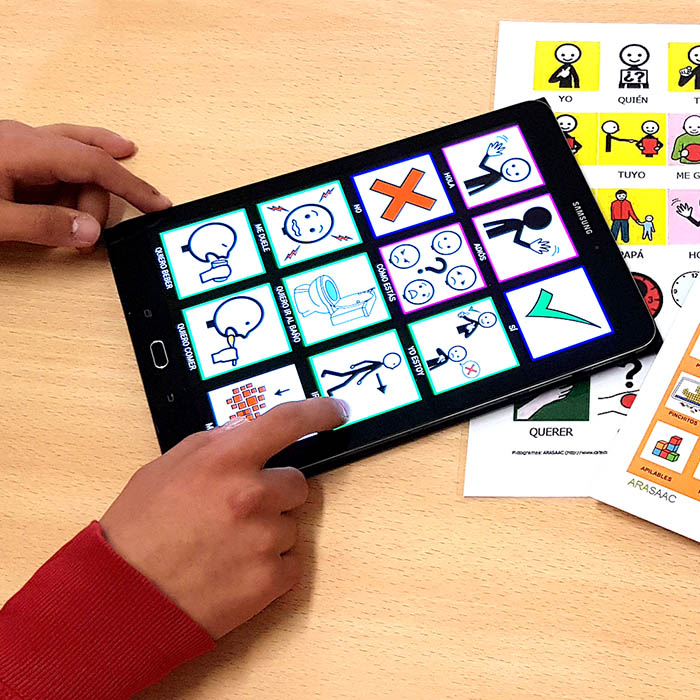
\includegraphics[width=0.45\textwidth]{img/pictos/tablero.jpg}
    \caption{Tablero de comunicación elaborado con pictogramas de ARASAAC. La persona usuaria señala los pictogramas en orden para formar un mensaje \cite{arasaac}}
    \label{fig:tablero}
\end{figure}

Esta segunda función es la que motiva la traducción automática de texto a pictogramas. En la práctica, preparar a mano una secuencia pictográfica para cada mensaje exige tiempo y conocimiento del catálogo, y eso limita la frecuencia con la que familiares, docentes o personal médico pueden usar pictogramas en una conversación real. Macaire et al.\ \cite{macaire2025overview} plantean la tarea Text-to-Picto justamente con este problema en mente: si un sistema es capaz de generar de forma automática una secuencia de pictogramas comprensible a partir de un enunciado, se facilita que la comunicación entre ambas partes se inicie sin depender de una preparación previa. En la edición 2025 de la tarea, además, se incorporaron enunciados del dominio médico junto con los de la vida cotidiana, lo cual refleja que uno de los escenarios de uso previstos es la comunicación entre pacientes y personal de salud.

\vspace{0.5cm}
\subsection{Redes Neuronales y Aprendizaje Profundo}
\vspace{0.2cm}

Una red neuronal artificial es un modelo compuesto por unidades de cálculo sencillas (neuronas) organizadas en capas. Cada neurona recibe un conjunto de entradas, calcula una suma ponderada de ellas, le agrega un sesgo y aplica una función de activación no lineal. Para una capa completa, esta operación se escribe de forma compacta como
\begin{equation}
\mathbf{h} = \sigma(\mathbf{W}\mathbf{x} + \mathbf{b}),
\end{equation}
donde $\mathbf{x}$ es el vector de entrada, $\mathbf{W}$ la matriz de pesos, $\mathbf{b}$ el vector de sesgos y $\sigma$ la función de activación (por ejemplo, ReLU o la tangente hiperbólica) \cite{goodfellow2016deep}. Sin la no linealidad, apilar capas equivaldría a aplicar una sola transformación lineal; es la función de activación la que permite que una red aproxime relaciones complejas entre entrada y salida.

Los pesos de la red no se diseñan a mano. Se ajustan a partir de ejemplos mediante la minimización de una función de pérdida que mide qué tan lejos está la predicción del valor esperado. El algoritmo que hizo práctico este ajuste en redes de varias capas fue la retropropagación del error, popularizada por Rumelhart, Hinton y Williams \cite{rumelhart1986learning}: el gradiente de la pérdida se calcula capa por capa, desde la salida hacia la entrada, aplicando la regla de la cadena, y luego se usa para actualizar los pesos con alguna variante del descenso por gradiente.


\subsubsection{Del aprendizaje superficial al profundo}


La idea de entrenar redes con muchas capas existía desde hace décadas, pero durante mucho tiempo resultó difícil llevarla a la práctica por falta de datos, de capacidad de cómputo y por problemas numéricos durante el entrenamiento. LeCun, Bengio y Hinton \cite{lecun2015deep} describen cómo esta situación cambió a partir de la década de 2010, cuando la disponibilidad de grandes conjuntos de datos, el uso de GPU y mejoras en inicialización y regularización permitieron entrenar redes profundas de forma estable. Lo que distingue al aprendizaje profundo, según estos autores, es que cada capa aprende una representación un poco más abstracta que la anterior, de modo que el modelo descubre por sí mismo las características relevantes que antes debían definirse manualmente.

En el caso del lenguaje, el reto particular es que los datos son secuencias de longitud variable en las que el orden importa. Las redes recurrentes atendieron este problema manteniendo un estado oculto que se actualiza con cada nuevo elemento, y las LSTM de Hochreiter y Schmidhuber \cite{hochreiter1997lstm} introdujeron compuertas que controlan qué información se conserva y cuál se descarta, lo que permitió aprender dependencias más largas que con una red recurrente simple. Como ya se describió en la sección anterior, estas arquitecturas dominaron el procesamiento de secuencias hasta la aparición de los mecanismos de atención y, después, del Transformer.


\subsubsection{Arquitectura Transformer}

El Transformer fue presentado por Vaswani et al.\ \cite{vaswani2017attention} en 2017 como un modelo de traducción automática que prescinde por completo de la recurrencia y de las convoluciones. En su lugar, cada posición de la secuencia se relaciona directamente con todas las demás mediante un mecanismo llamado autoatención (\textit{self-attention}). El trabajo mostró que esta arquitectura obtenía mejores resultados que los sistemas recurrentes de la época en las tareas de traducción inglés-alemán e inglés-francés de WMT 2014, con un costo de entrenamiento menor gracias a que las operaciones pueden paralelizarse.


\subsubsection{Atención de producto punto escalado}


La pieza básica del modelo es la atención de producto punto escalado. Cada token de la entrada se proyecta en tres vectores: una consulta ($q$), una clave ($k$) y un valor ($v$). Intuitivamente, la consulta expresa ``qué busca'' un token, la clave indica ``qué ofrece'' cada token y el valor es la información que efectivamente se transmite. Agrupando estos vectores en las matrices $Q$, $K$ y $V$, la atención se calcula como
\begin{equation}
\text{Attention}(Q, K, V) = \text{softmax}\left(\frac{QK^{\top}}{\sqrt{d_k}}\right)V,
\end{equation}
donde $d_k$ es la dimensión de las claves \cite{vaswani2017attention}. El producto $QK^{\top}$ mide la afinidad entre cada par de tokens, la función softmax convierte esas afinidades en pesos que suman uno, y el resultado es un promedio ponderado de los valores. La división entre $\sqrt{d_k}$ evita que los productos punto crezcan demasiado cuando la dimensión es grande, lo que llevaría a la softmax a regiones con gradientes muy pequeños.

En lugar de calcular una sola atención, el Transformer utiliza atención multicabeza: repite el cálculo anterior $h$ veces en paralelo con proyecciones distintas y concatena los resultados. Cada cabeza puede especializarse en un tipo de relación diferente, por ejemplo, una puede vincular un verbo con su sujeto y otra un pronombre con su referente.


\subsubsection{Codificador, decodificador y codificación posicional}


El modelo original sigue el esquema codificador-decodificador. El codificador está formado por una pila de capas idénticas, cada una con un bloque de autoatención multicabeza y una red \textit{feed-forward} aplicada a cada posición, ambos rodeados por conexiones residuales y normalización de capa. El decodificador tiene una estructura similar, con dos diferencias: su autoatención está enmascarada para que cada posición solo pueda ver los tokens ya generados, y añade un bloque de atención cruzada en el que las consultas provienen del decodificador y las claves y valores de la salida del codificador. Es en esta atención cruzada donde el modelo ``consulta'' la oración de origen mientras genera la de destino \cite{vaswani2017attention}.

Como la autoatención trata la entrada como un conjunto y no distingue el orden, los autores sumaron a cada embedding una codificación posicional construida con funciones seno y coseno de distintas frecuencias:
\begin{equation}
PE_{(pos, 2i)} = \sin\left(\frac{pos}{10000^{2i/d_{\text{model}}}}\right), \qquad
PE_{(pos, 2i+1)} = \cos\left(\frac{pos}{10000^{2i/d_{\text{model}}}}\right).
\end{equation}
De esta manera cada posición recibe una firma única y el modelo puede razonar sobre distancias relativas entre tokens \cite{vaswani2017attention}.

\vspace{0.5cm}
\subsection{Modelos Preentrenados y Transfer Learning}
\vspace{0.2cm}

El aprendizaje por transferencia (\textit{transfer learning}) parte de la noción de que, el conocimiento adquirido al resolver una tarea puede aprovecharse para resolver otra distinta pero relacionada. Pan y Yang \cite{pan2010survey} formalizan esta idea en términos de un dominio y una tarea de origen, de los que se extrae conocimiento, y un dominio y una tarea de destino, en los que se aplica. Su utilidad es mayor cuando la tarea de destino cuenta con pocos datos etiquetados, que es la situación habitual en problemas especializados.

En el procesamiento de lenguaje natural esta idea tomó la forma de un procedimiento en dos etapas. Primero, un modelo se \textit{preentrena} sobre grandes cantidades de texto sin etiquetar con un objetivo autosupervisado, como predecir palabras ocultas o la siguiente palabra. Después, ese mismo modelo se \textit{ajusta finamente} (\textit{fine-tuning}) con un conjunto de datos pequeño y etiquetado de la tarea que interesa. Uno de los trabajos que mostró que este esquema funcionaba en lenguaje natural fue ULMFiT (\textit{Universal Language Model Fine-tuning}), propuesto por Howard y Ruder \cite{howard2018ulmfit}. Su punto de partida es un modelo de lenguaje recurrente basado en LSTM, preentrenado sobre un corpus general extraído de Wikipedia para predecir la siguiente palabra. El método ajusta ese modelo en tres etapas: primero el preentrenamiento general, después un ajuste del modelo de lenguaje con texto del dominio de destino (aún sin etiquetas) y, por último, el ajuste como clasificador con los datos etiquetados. Con este procedimiento mostraron que con solo 100 ejemplos etiquetados se igualaba el desempeño de un modelo entrenado desde cero con cien veces más datos.


\subsubsection{Modelos preentrenados basados en Transformer}


La combinación del preentrenamiento con la arquitectura Transformer dio lugar a una familia de modelos que se convirtió en el punto de partida estándar del campo. BERT \cite{devlin2019bert} utiliza solo el codificador y se preentrena ocultando al azar una parte de los tokens de entrada para que el modelo los reconstruya a partir del contexto de ambos lados. Esto lo hace muy adecuado para tareas de comprensión, como clasificación o reconocimiento de entidades, pero no está pensado para generar texto.

Para tareas en las que la salida es una secuencia nueva, como la traducción, resultan más naturales los modelos que conservan el esquema completo codificador-decodificador. BART \cite{lewis2020bart} se preentrena corrompiendo el texto de entrada (borrando, enmascarando o desordenando fragmentos) y enseñando al modelo a recuperar el texto original. T5 \cite{raffel2020t5}, por su parte, parte de la propuesta de tratar cualquier problema de lenguaje como una conversión de texto a texto: la entrada es una cadena precedida por un prefijo que indica la tarea (por ejemplo, \textit{translate English to German:}) y la salida es otra cadena. Raffel et al.\ realizaron además un estudio sistemático comparando objetivos de preentrenamiento, arquitecturas y tamaños de modelo, lo que hizo de T5 una referencia útil para entender qué decisiones de diseño importan en la práctica. FLAN-T5 \cite{chung2022flan} extiende T5 con un ajuste adicional sobre una colección amplia de tareas formuladas como instrucciones, lo cual mejora su comportamiento cuando se enfrenta a tareas nuevas.

Estos modelos codificador-decodificador son relevantes para el presente trabajo porque son, en su mayoría, la base de los sistemas que han participado en la tarea Text-to-Picto, como se describe en el capítulo~\ref{sec:estado-arte}.

\vspace{0.5cm}
\subsection{Traducción Automática con Transformers}
\vspace{0.2cm}

La traducción automática neuronal formula el problema de traducir como el de modelar la probabilidad de una oración destino $\mathbf{y} = (y_1, \dots, y_m)$ dada una oración origen $\mathbf{x}$. Esta probabilidad se descompone de forma autorregresiva, es decir, cada token se predice a partir de la oración de origen y de los tokens ya generados:
\begin{equation}
P(\mathbf{y} \mid \mathbf{x}) = \prod_{t=1}^{m} P(y_t \mid y_{<t}, \mathbf{x}).
\end{equation}
Sutskever, Vinyals y Le \cite{sutskever2014sequence} mostraron que este esquema podía implementarse con dos redes LSTM, una que codifica la oración de origen en un vector de tamaño fijo y otra que genera la traducción a partir de él. El problema de comprimir toda la oración en un solo vector se hacía evidente con oraciones largas, y Bahdanau, Cho y Bengio \cite{bahdanau2015neural} lo atenuaron permitiendo que el decodificador consultara, en cada paso, una combinación ponderada de todos los estados del codificador. Ese mecanismo de atención es el antecedente directo del Transformer, que llevó la misma idea a todas las capas del modelo y eliminó la recurrencia \cite{vaswani2017attention}.


\subsubsection{Entrenamiento y decodificación}


Un modelo Transformer de traducción se entrena con pares de oraciones alineadas, minimizando la entropía cruzada entre la distribución que predice el modelo y el token correcto de la referencia en cada posición. Durante el entrenamiento se usa la técnica de \textit{teacher forcing}: el decodificador recibe como entrada los tokens verdaderos de la referencia y no los que él mismo generó, lo que permite procesar toda la oración en paralelo gracias a la máscara de atención.

Al momento de traducir ya no se dispone de la referencia, por lo que la salida debe construirse token por token. La estrategia más simple, la decodificación voraz, elige en cada paso el token más probable, pero puede comprometerse con una elección temprana que después resulte mala. Por ello es común usar búsqueda en haz (\textit{beam search}), que mantiene en paralelo las $k$ hipótesis parciales más probables y al final selecciona la de mayor probabilidad total \cite{sutskever2014sequence}.

Un último elemento práctico es el vocabulario. Los sistemas modernos no trabajan con palabras completas sino con unidades de subpalabra obtenidas con algoritmos como Byte Pair Encoding \cite{sennrich2016bpe} o SentencePiece. Esto permite representar palabras raras o nunca vistas como combinaciones de fragmentos conocidos, con un vocabulario de tamaño controlado.


\subsubsection{Relación con la traducción a pictogramas}

La traducción de texto a pictogramas puede plantearse con exactamente el mismo esquema: la oración de origen es el texto en lenguaje natural y la secuencia destino está formada por términos pictográficos de ARASAAC \cite{macaire2025overview}. Esto permite reutilizar modelos preentrenados como T5 o BART y ajustarlos con los pares texto-pictograma del conjunto de datos de la tarea.

Sin embargo, la adaptación tiene particularidades. El lenguaje de destino es más reducido que un idioma natural, ya que carece de flexiones y de la mayoría de las palabras funcionales, así que la tarea consiste en buena medida en decidir qué conceptos conservar, cómo normalizarlos a su forma canónica y en qué orden presentarlos. Además, el vocabulario de salida es cerrado, lo que abre la posibilidad de restringir la generación a términos que efectivamente existan en el catálogo.


\subsection{Métricas de Evaluación en Traducción Automática}
La evaluación de sistemas de Traducción Automática (MT, por sus siglas en inglés) constituye un componente metodológico indispensable para el avance del campo, dado que permite comparar de forma objetiva el desempeño de distintas arquitecturas y determinar el grado de proximidad entre una traducción generada por un sistema y una traducción de referencia producida por un humano. Históricamente, la evaluación humana ha sido considerada el estándar de referencia por su capacidad de capturar matices semánticos, fluidez y adecuación que resultan difíciles de cuantificar computacionalmente; sin embargo, este tipo de evaluación presenta limitaciones sustanciales: es costosa en tiempo y recursos, difícil de escalar a grandes volúmenes de datos, y susceptible a variabilidad, lo que termina por afectar su reproducibilidad \cite{lee2023survey}.

Estas limitaciones motivaron el desarrollo de métricas automáticas que aproximan el juicio humano mediante el análisis de similitud léxica, sintáctica o semántica entre la hipótesis generada por el sistema y una o más referencias. El auge de la arquitectura \textit{Transformer} y la consecuente mejora sustancial en la calidad de las traducciones producidas por sistemas neuronales han intensificado la necesidad de contar con métricas automáticas confiables que permitan monitorear el progreso del campo sin depender exclusivamente de evaluación humana \cite{lee2023survey}. No obstante, evaluar y comparar sistemas de MT de forma automática continúa siendo una tarea no trivial: diversas métricas tradicionales, entre ellas BLEU y TER, han mostrado un desempeño limitado para capturar similitud semántica entre las salidas de los sistemas y las referencias humanas, lo cual ha impulsado tanto el refinamiento de métricas léxicas como el desarrollo de métricas basadas en representaciones neuronales \cite{lee2023survey}. Pese a estas limitaciones, las métricas automáticas basadas en superposición léxica mantienen vigencia dentro de la investigación en MT por su bajo costo computacional, su interpretabilidad y la posibilidad de comparabilidad directa con resultados reportados en trabajos previos.


\subsubsection{Relación con la traducción automática a pictogramas}


La traducción automática a pictogramas comparte con la MT convencional su formulación fundamental como un problema de \textit{sequence-to-sequence}: esto quiere decir que dado un enunciado de entrada, el sistema debe producir una secuencia de salida que preserve el contenido semántico del origen. En consecuencia, los desafíos de evaluación inherentes a la MT se trasladan directamente a la evaluación de sistemas de traducción a pictogramas.

Existen, sin embargo, diferencias sustanciales entre ambas tareas que condicionan la aplicabilidad directa de las métricas de MT. En primer lugar, el espacio de salida en la traducción a pictogramas no es lenguaje natural sino una secuencia de tokens discretos, cada uno vinculado a un pictograma perteneciente a un vocabulario cerrado (por ejemplo, el catálogo ARASAAC), lo cual reduce la variabilidad morfológica y sintáctica presente en el texto libre. En segundo lugar, los pictogramas no cambian de forma según el género, número o tiempo verbal (por ejemplo, no existe una versión distinta de un pictograma para «corrió» frente a «correrá»), y tampoco incluyen palabras funcionales como artículos, preposiciones o conjunciones («el», «de», «y»). Esto significa que aspectos que en la traducción automática de texto son muy importantes de evaluar (tales como el orden de las palabras o que las palabras concuerden entre sí en género y número) tienen una relevancia distinta cuando se trata de evaluar secuencias de pictogramas.

Pese a estas diferencias, resulta razonable adaptar las métricas originalmente diseñadas para MT a la tarea de traducción a pictogramas, dado que ambas comparten la necesidad de cuantificar la distancia entre una secuencia generada y una secuencia de referencia mediante superposición de unidades (n-gramas, tokens o ediciones). La principal ventaja de esta adaptación es la posibilidad de aprovechar métricas ya validadas y ampliamente adoptadas por la comunidad de MT, lo que favorece la comparabilidad de resultados entre sistemas. La principal limitación radica en que estas métricas fueron diseñadas y calibradas sobre corpus de lenguaje natural, por lo que su correlación con juicios humanos de calidad en el dominio pictográfico no está garantizada de forma automática y debe complementarse, como se discutirá más adelante, con métricas diseñadas específicamente para operar sobre el vocabulario pictográfico.

\subsubsection{BLEU}
\vspace{-0.1cm}
\begin{itemize}
\item \textit{Fundamentos} \\
\vspace{-0.5cm}

BLEU (Bilingual Evaluation Understudy) fue propuesta por \citet{papineni2002bleu} como respuesta a la necesidad de una métrica automática, rápida y de bajo costo que correlacionara razonablemente con el juicio humano, evitando la dependencia de evaluación manual extensiva. La motivación central de BLEU es que una traducción automática será considerada de mayor calidad en la medida en que comparta más n-gramas contiguos con una o varias traducciones de referencia producidas por humanos.

\item \textit{Funcionamiento}\\
\vspace{-0.5cm}

El cálculo de BLEU parte de la tokenización de la hipótesis y de la(s) referencia(s). Sobre el texto tokenizado se extraen n-gramas de orden $1$ a $N$ (típicamente $N=4$). Para cada orden $n$, se calcula la \textit{precisión de n-gramas modificada} ($p_n$), la cual difiere de la precisión estándar en que el conteo de coincidencias de cada n-grama se \textit{recorta} (clipping) al número máximo de veces que dicho n-grama aparece en cualquiera de las referencias, evitando así que un sistema obtenga una puntuación artificialmente alta repitiendo n-gramas de alta frecuencia.

Dado que la precisión de n-gramas tiende a favorecer traducciones más cortas que la referencia (al reducir la probabilidad de introducir n-gramas no coincidentes), BLEU incorpora una \textit{penalización por brevedad} (Brevity Penalty, BP) que castiga hipótesis sustancialmente más cortas que la referencia.

\item\textit{Formulación matemática} \\
\vspace{-0.5cm}

La precisión de n-gramas modificada se define como:

\begin{equation}
p_n = \frac{\sum_{C \in \{\text{Candidatos}\}} \sum_{n\text{-grama} \in C} \text{Count}_{\text{clip}}(n\text{-grama})}{\sum_{C' \in \{\text{Candidatos}\}} \sum_{n\text{-grama}' \in C'} \text{Count}(n\text{-grama}')}
\end{equation}

donde $\text{Count}_{\text{clip}}$ es el conteo de coincidencias recortado al máximo número de ocurrencias del n-grama en cualquier referencia. La penalización por brevedad se define como:

\begin{equation}
BP =
\begin{cases}
1 & \text{si } c > r \\
e^{(1 - r/c)} & \text{si } c \leq r
\end{cases}
\end{equation}

donde $c$ es la longitud de la hipótesis y $r$ es la longitud efectiva de la referencia (usualmente la de longitud más cercana a $c$). Finalmente, BLEU se calcula como:

\begin{equation}
\text{BLEU} = BP \cdot \exp\left(\sum_{n=1}^{N} w_n \log p_n\right)
\end{equation}

con $w_n$ los pesos asignados a cada orden de n-grama, típicamente uniformes ($w_n = 1/N$) \cite{papineni2002bleu}.

\item \textit{Ejemplo detallado} \\
\vspace{-0.5cm}

Sea la referencia: \textit{``el gato está sobre la alfombra''} y la hipótesis: \textit{``el gato está en la alfombra''}.

Para unigramas ($n=1$): la hipótesis tiene 6 tokens; de estos, coinciden con la referencia (con clipping) 5 (\textit{el, gato, está, la, alfombra}), por lo que $p_1 = 5/6$.

Para bigramas ($n=2$): los bigramas de la hipótesis son (el-gato, gato-está, está-en, en-la, la-alfombra); de estos coinciden con la referencia (el-gato, gato-está, la-alfombra), es decir 3 de 5, por lo que $p_2 = 3/5$.

Continuando de forma análoga para $n=3$ y $n=4$, y dado que $c = r = 6$ (BP = 1 pues $c = r$, no $c < r$), el valor final de BLEU se obtiene promediando geométricamente los $p_n$ ponderados y multiplicando por BP. Este ejemplo ilustra cómo un solo token distinto (``en'' en lugar de ``sobre'') degrada progresivamente más la puntuación conforme aumenta el orden del n-grama, ya que afecta a más n-gramas contiguos.

\item \textit{Interpretación} \\
\vspace{-0.5cm}

BLEU se expresa típicamente en una escala de 0 a 100 (o 0 a 1). Valores cercanos a 100 indican alta coincidencia léxica con la referencia; en la práctica, puntuaciones por encima de 30 suelen considerarse indicativas de una traducción comprensible, mientras que puntuaciones por encima de 50 se asocian con traducciones de alta calidad, aunque estos umbrales varían considerablemente según el par de idiomas y el dominio.

\item \textit{Ventajas}\\
\vspace{-0.5cm}

BLEU es computacionalmente eficiente, no requiere entrenamiento ni recursos lingüísticos adicionales, y ha sido validada extensamente por su correlación razonable con juicios humanos a nivel de corpus, lo que ha consolidado su uso como métrica de referencia en la literatura de MT durante más de dos décadas.

\item \textit{Limitaciones} \\
\vspace{-0.5cm}

BLEU no captura equivalencia semántica (penaliza sinónimos y paráfrasis válidas), es sensible a la tokenización empleada (lo cual compromete la reproducibilidad entre estudios si no se estandariza) \cite{lee2023survey}, y su correlación con juicios humanos es más débil a nivel de oración individual que a nivel de corpus completo.

\item \textit{Aplicación a traducción de pictogramas}\\
\vspace{-0.5cm}

En el contexto de traducción a pictogramas, BLEU puede aplicarse directamente sobre la secuencia de tokens pictográficos (en lugar de palabras), tratando cada identificador de pictograma como una unidad léxica. Esto permite capturar coincidencias exactas de secuencias de pictogramas, pero hereda la limitación de no reconocer equivalencias semánticas entre pictogramas distintos que podrían transmitir un significado similar dentro del vocabulario ARASAAC.
\end{itemize}


\subsubsection{METEOR}

\begin{itemize}
\item \textit{Fundamentos} \\
\vspace{-0.5cm}

METEOR (Metric for Evaluation of Translation with Explicit ORdering) fue propuesta por \citet{banerjee2005meteor} para abordar limitaciones específicas de BLEU, particularmente su insensibilidad al orden de palabras a nivel de oración y su incapacidad de reconocer coincidencias no exactas (sinónimos, variantes morfológicas). La motivación central es construir una métrica que se correlacione mejor con el juicio humano combinando precisión y \textit{recall}, en lugar de basarse exclusivamente en precisión de n-gramas.

\item \textit{Funcionamiento} \\
\vspace{-0.5cm}

METEOR alinea unigramas entre hipótesis y referencia mediante un proceso de emparejamiento en etapas sucesivas: primero coincidencias exactas, después coincidencias tras normalización morfológica (\textit{stemming}), y finalmente coincidencias de sinónimos mediante recursos léxicos externos (como WordNet, en la versión original para inglés). A partir del conjunto de unigramas alineados se calculan precisión ($P$) y \textit{recall} ($R$), que se combinan en una media armónica ponderada. Adicionalmente, METEOR agrupa los unigramas alineados en \textit{chunks} (bloques contiguos y ordenados de igual manera en ambas secuencias) y penaliza la fragmentación excesiva, capturando así, de forma indirecta, el orden de palabras.

\item \textit{Formulación matemática}\\
\vspace{-0.5cm}

La media armónica ponderada (F-mean), con fuerte sesgo hacia el recall, se define como:

\begin{equation}
F_{\text{mean}} = \frac{10 \cdot P \cdot R}{R + 9P}
\end{equation}

correspondiente al caso en que el parámetro $\alpha = 0.9$ en la forma general $F_{\text{mean}} = \frac{P \cdot R}{\alpha P + (1-\alpha) R}$. La penalización por fragmentación se calcula como:

\begin{equation}
\text{Penalty} = \gamma \left(\frac{ch}{m}\right)^{\beta}
\end{equation}

donde $ch$ es el número de \textit{chunks}, $m$ es el número total de unigramas alineados, y $\gamma$, $\beta$ son parámetros ajustables (comúnmente $\gamma = 0.5$, $\beta = 3$) \cite{banerjee2005meteor}. El puntaje final es:

\begin{equation}
\text{METEOR} = F_{\text{mean}} \cdot (1 - \text{Penalty})
\end{equation}


\item \textit{Ejemplo detallado} \\
\vspace{-0.5cm}

Retomando el ejemplo anterior: referencia \textit{``el gato está sobre la alfombra''} (6 unigramas) e hipótesis \textit{``el gato está en la alfombra''} (6 unigramas). Los unigramas alineados exactamente son 5 (\textit{el, gato, está, la, alfombra}), por lo que $P = 5/6$ y $R = 5/6$. Aplicando la fórmula de $F_{\text{mean}}$ con estos valores iguales, $F_{\text{mean}} = 5/6 \approx 0.833$. Dado que los unigramas alineados forman en su mayoría un único chunk contiguo (con una pequeña discontinuidad en el punto donde ``en'' reemplaza a ``sobre''), la penalización por fragmentación resulta baja, de modo que el puntaje final se aproxima a $F_{\text{mean}}$, quedando ligeramente por debajo de 0.833 tras aplicar la penalización.

\item \textit{Interpretación} \\
\vspace{-0.5cm}

METEOR se reporta en una escala de 0 a 100 (o 0 a 1); valores más altos indican mayor calidad de traducción. A diferencia de BLEU, sus valores tienden a ser numéricamente más altos para una misma traducción debido al sesgo hacia recall y al reconocimiento de coincidencias no exactas, por lo que los umbrales de referencia no son directamente comparables entre ambas métricas.

\item \textit{Ventajas} \\
\vspace{-0.5cm}


METEOR incorpora información semántica adicional no capturada por BLEU y considera explícitamente el orden de palabras mediante la penalización por fragmentación, lo cual mejora su correlación con juicios humanos a nivel de oración \cite{lee2023survey}.

\item \textit{Limitaciones} \\
\vspace{-0.5cm}

La dependencia de recursos léxicos externos (como WordNet) limita su aplicabilidad directa a idiomas o dominios donde dichos recursos son escasos o inexistentes; además, los parámetros $\alpha$, $\gamma$ y $\beta$ requieren calibración específica por idioma para un desempeño óptimo.

\item \textit{Aplicación a traducción de pictogramas} \\
\vspace{-0.5cm}

Aplicar METEOR a secuencias de pictogramas requiere redefinir la noción de ``sinónimo'' en términos del vocabulario pictográfico, dado que no existe un recurso léxico equivalente a WordNet para pictogramas ARASAAC. En ausencia de dicho recurso, la aplicación práctica de METEOR en este dominio suele limitarse a coincidencias exactas de identificadores de pictograma, lo que reduce su ventaja teórica frente a BLEU pero conserva su capacidad de penalizar fragmentación en el orden de la secuencia.
\end{itemize}

\subsubsection{TER}
\vspace{-0.1cm}
\begin{itemize}
\item \textit{Fundamentos} \\
\vspace{-0.5cm}

TER (Translation Edit Rate) fue propuesta por \citet{snover2006ter} con la motivación de cuantificar directamente el esfuerzo humano requerido para corregir una traducción automática hasta que coincida con una referencia, en lugar de medir superposición de n-gramas. Esta orientación hace de TER una métrica particularmente interpretable en contextos de posedición.

\item \textit{Funcionamiento} \\
\vspace{-0.5cm}

TER calcula el número mínimo de operaciones de edición (inserciones, eliminaciones, sustituciones y desplazamientos de bloques de palabras) necesarias para transformar la hipótesis en la referencia, mediante una variante del algoritmo de distancia de edición de Levenshtein extendida con la operación de desplazamiento (\textit{shift}), que permite reordenar secuencias completas de palabras con un costo unitario, reconociendo que distintos órdenes de palabras pueden ser igualmente válidos en muchos idiomas \cite{snover2006ter}.

\item \textit{Formulación matemática} \\
\vspace{-0.5cm}

\begin{equation}
\text{TER} = \frac{\text{\footnotesize No. de ediciones (inserciones + eliminaciones + sustituciones + desplazamientos)}}{\text{\footnotesize Número promedio de palabras en la(s) referencia(s)}}
\end{equation}

 A diferencia de BLEU y METEOR, TER es una métrica de \textit{error}, por lo que valores más bajos indican mejor calidad de traducción.

\item \textit{Ejemplo detallado} \\
\vspace{-0.5cm}

Con el mismo par (referencia de 6 palabras, hipótesis con una sustitución: ``en'' por ``sobre''), se requiere una única operación de edición (sustitución) para transformar la hipótesis en la referencia. Por lo tanto:

\begin{equation}
\text{TER} = \frac{1}{6} \approx 0.167 \; (16.7\%)
\end{equation}

lo que indica que, en promedio, un 16.7\% de las palabras de la referencia requirieron edición para reconstruirse a partir de la hipótesis.

\item \textit{Interpretación} \\
\vspace{-0.5cm}

Al ser una métrica de error, valores cercanos a 0 indican traducciones que requieren mínima edición (alta calidad), mientras que valores cercanos o superiores a 1 indican que la hipótesis requiere un número de ediciones comparable o mayor a la longitud total de la referencia.

\item \textit{Ventajas} \\
\vspace{-0.5cm}

TER es intuitivamente interpretable en términos de esfuerzo de posedición y su variante orientada a humanos (HTER) ha mostrado una correlación con juicios humanos comparable o superior a la de un segundo juicio humano independiente \cite{snover2006ter}.

\item \textit{Limitaciones} \\
\vspace{-0.5cm}

TER, al igual que BLEU, opera a nivel de superposición léxica exacta y no reconoce sinónimos o paráfrasis; además, el costo computacional del cálculo de la operación de desplazamiento es superior al de una distancia de edición estándar.


\item \textit{Aplicación a traducción de pictogramas}


TER resulta directamente aplicable a secuencias de pictogramas al tratar cada identificador de pictograma como una unidad editable, y su naturaleza basada en operaciones de edición la aproxima conceptualmente a PictoER, una métrica derivada de Word Error Rate y adoptada específicamente en la evaluación de sistemas de traducción a pictogramas, que desplaza la unidad de análisis de la palabra al token pictográfico para capturar con mayor precisión el tipo de error relevante en este dominio.
\end{itemize}


\subsubsection{chrF y chrF++}
\label{par:chrf}
\vspace{-0.1cm}
\begin{itemize}
\item \textit{Fundamentos} \\
\vspace{-0.5cm}
 
chrF (\textit{character n-gram F-score}) fue propuesta por \citet{popovic2015chrf} como una métrica automática que compara la hipótesis y la referencia a nivel de caracteres, no de palabras. La motivación es que BLEU trata como error total a dos palabras que solo difieren en una terminación, como \textit{gato} y \textit{gatos}. Al trabajar con caracteres, chrF reconoce coincidencias parciales, lo que la hace más adecuada para idiomas con mucha variación morfológica. Más tarde, \citet{popovic2017chrfpp} propuso chrF++, que añade a los n-gramas de caracteres los unigramas y bigramas de palabras.
 
\item \textit{Funcionamiento} \\
\vspace{-0.5cm}
 
Se extraen los n-gramas de caracteres de la hipótesis y de la referencia, normalmente de orden 1 a 6, sin contar los espacios. Para cada orden se calcula la precisión (qué parte de los n-gramas de la hipótesis aparece en la referencia) y el \textit{recall} (qué parte de los n-gramas de la referencia aparece en la hipótesis). Después se promedian los valores de todos los órdenes y se combinan en una F-score que da más peso al \textit{recall}. En chrF++ se hace lo mismo, pero también se incluyen n-gramas de palabras de orden 1 y 2.
 
\item \textit{Formulación matemática} \\
\vspace{-0.5cm}
 
Sean $\text{chrP}$ y $\text{chrR}$ la precisión y el \textit{recall} promedio de los n-gramas considerados. La métrica es:
 
\begin{equation}
\text{chrF}_{\beta} = (1+\beta^2)\,\frac{\text{chrP} \cdot \text{chrR}}{\beta^2 \cdot \text{chrP} + \text{chrR}}
\end{equation}
 
donde $\beta$ indica cuántas veces más importa el \textit{recall} que la precisión. El valor usual es $\beta = 2$ \cite{popovic2015chrf}. chrF++ usa la misma fórmula, pero el promedio incluye los n-gramas de caracteres de orden 1 a 6 y los de palabras de orden 1 a 2 \cite{popovic2017chrfpp}.
 
\item \textit{Ejemplo detallado} \\
\vspace{-0.5cm}
 
Sea la referencia \textit{``gato''} y la hipótesis \textit{``gatos''}. Para simplificar, se usan solo bigramas de caracteres. La referencia tiene 3 bigramas (\textit{ga, at, to}) y la hipótesis tiene 4 (\textit{ga, at, to, os}). Coinciden 3, por lo que la precisión es $3/4 = 0.75$ y el \textit{recall} es $3/3 = 1$. Con $\beta = 2$:
 
\begin{equation}
\text{chrF}_2 = 5 \cdot \frac{0.75 \cdot 1}{4 \cdot 0.75 + 1} = \frac{3.75}{4} \approx 0.94
\end{equation}
 
A nivel de palabra, BLEU no encontraría ninguna coincidencia entre \textit{gato} y \textit{gatos}. chrF, en cambio, reconoce que la hipótesis es casi correcta.
 
\item \textit{Interpretación} \\
\vspace{-0.5cm}
 
chrF++ se reporta en una escala de 0 a 100. Valores más altos indican que la hipótesis se parece más a la referencia. Como BLEU, sus valores solo son comparables entre sistemas evaluados sobre el mismo idioma y el mismo conjunto de prueba.
 
\item \textit{Ventajas} \\
\vspace{-0.5cm}
 
No depende de la tokenización en palabras, reconoce variantes morfológicas y no necesita recursos lingüísticos externos. Por eso se usa para reportar resultados en conjuntos con muchos idiomas, como FLORES-200 \cite{nllbteamNoLanguageLeft2022}.
 
\item \textit{Limitaciones} \\
\vspace{-0.5cm}
 
Sigue midiendo parecido superficial: no reconoce sinónimos ni paráfrasis. Además, sus valores dependen del sistema de escritura. En idiomas que no separan las palabras con espacios, como el japonés o el chino, los valores son mucho más bajos aunque la traducción sea buena, por lo que no sirve para comparar la calidad entre idiomas con escrituras distintas.
 
    
\end{itemize}
 
 
\subsubsection{CometKiwi}
\label{par:cometkiwi}
\vspace{-0.1cm}
\begin{itemize}
\item \textit{Fundamentos} \\
\vspace{-0.5cm}
 
CometKiwi fue propuesta por \citet{rei2022cometkiwi} como una métrica de \textit{estimación de calidad} (\textit{quality estimation}). A diferencia de BLEU, METEOR, TER o chrF++, no necesita una traducción de referencia: estima qué tan buena es una traducción usando solo la oración fuente y la traducción. La motivación es que en muchos casos reales no existen traducciones humanas con las cuales comparar, y aun así se necesita saber si una traducción automática es confiable.
 
\item \textit{Funcionamiento} \\
\vspace{-0.5cm}
 
CometKiwi es una red neuronal basada en un codificador Transformer multilingüe preentrenado. La oración fuente y su traducción se unen en una sola entrada y el codificador las procesa juntas, de modo que puede relacionar cada parte de la traducción con la parte correspondiente del original. La representación resultante pasa por una red \textit{feed-forward} que produce un solo número: la calidad estimada. El modelo se entrenó para imitar calificaciones que asignaron evaluadores humanos a miles de traducciones (\textit{direct assessments}) \cite{rei2022cometkiwi}.
 
\item \textit{Formulación matemática} \\
\vspace{-0.5cm}
 
Sea $s$ la oración fuente y $t$ su traducción. El codificador produce una representación conjunta $\mathbf{h} = \text{Enc}([s; t])$, y la calidad estimada es:
 
\begin{equation}
\hat{y} = \text{FFN}(\mathbf{h})
\end{equation}
 
Durante el entrenamiento se minimiza el error cuadrático medio entre $\hat{y}$ y la calificación humana $y$:
 
\begin{equation}
\mathcal{L} = \frac{1}{M}\sum_{i=1}^{M}\left(\hat{y}_i - y_i\right)^2
\end{equation}
 
donde $M$ es el número de pares de entrenamiento.
 
\item \textit{Ejemplo detallado} \\
\vspace{-0.5cm}
 
Sea la fuente en francés \textit{``le chat est sur le tapis''}. Si la traducción al español es \textit{``el gato está sobre la alfombra''}, el modelo reconoce que el contenido se conserva y asigna un valor alto. Si la traducción es \textit{``el gato está''}, el modelo detecta que falta información del original y asigna un valor más bajo, aunque lo que sí se tradujo sea correcto. Esto no se puede medir con chrF++ sin una traducción de referencia.
 
\item \textit{Interpretación} \\
\vspace{-0.5cm}
 
La versión \texttt{wmt22-cometkiwi-da} produce valores aproximadamente entre 0 y 1; valores más altos indican mayor calidad estimada. Como el modelo evalúa el significado y no la forma escrita, sus valores sí se pueden comparar entre idiomas con sistemas de escritura distintos.
 
\item \textit{Ventajas} \\
\vspace{-0.5cm}
 
No necesita referencias, captura equivalencias de significado (sinónimos, paráfrasis, cambios de orden) y funciona para los idiomas que cubre su codificador multilingüe.
 
\item \textit{Limitaciones} \\
\vspace{-0.5cm}
 
Su resultado no es interpretable: da un número, pero no explica qué error encontró. Requiere una GPU para evaluar volúmenes grandes de texto. Además, es menos confiable con oraciones muy cortas, porque tiene poco contexto para juzgar.

\end{itemize}
